\section{Results}
\label{sec:results}


\subsection{Infection estimates reveal waves missed by reported cases}
\label{sec:omitted-waves}

Outbreaks in infections precede those in reported cases and are reliably larger
in magnitude. But simply shifting cases back in time and increasing them by some
factor fails to capture the spatio-temporal dynamics of the pandemic. 
Hence, relative to reported cases, examining estimated infections reveals a
rather different pattern. \autoref{fig:state_infect_est} shows
estimates of the number of daily new infections per 100,000 inhabitants for each
\US state from June 1, 2020 to November 29, 2021 compared with reported cases,
and deconvolved cases (reported cases ``pushed back'' by the delays shown in
\autoref{fig:chain_events_onset_report}). 

While the major Ancestral, Alpha, and Delta waves tend to be visible for most
states, there are clear outbreaks in unreported infections that are not easily
detectable from cases alone in the falls of 2020 and 2021. For example, a wave
of infections is present in the spring of 2021 for North Dakota and South Dakota
which is not visible in reported cases alone. For the specific date of Oct. 20,
2020, \autoref{fig:choro_inf_case_rates} shows heightened case rates in the
northern states like North Dakota, South Dakota, and Wisconsin relative to other
states. However, the infection rates more clearly shows that the influx in
infections is not limited to these states, but extends out to the surrounding
states. Later in the pandemic, the fall of 2021, we can see that the major Delta
wave is only faintly detectable from cases in a number of eastern states such as
Maryland and Connecticut. It is clear that cases fail to adequately capture the
rise and fall in infections during this time.

\subsection{The cases/infections ratio varies by state and variant.}
\label{sec:case-infection-ratio}

While it is clear from \autoref{fig:state_infect_est} that cases underestimate
the true burden of infections for every state, the degree to which this problem
persists varies across states and variants. For the major Delta wave, some of
the greatest discrepancies between cases and infections are visible in the
Western states of Idaho and Montana, the Southern states of Louisiana and
Georgia, and the Midwestern states of Iowa and Nebraska. In addition, we can see
that the Delta wave is only faintly detectable from cases in a number of Eastern
states (e.g., Maryland and Connecticut). The Ancestral wave is poorly
represented \attn{what does ``poorly represented'' mean} by cases in several
midwestern states (take, for example, Illinois, Indiana, and Ohio). Earlier on
in the pandemic, such discrepancies between cases and infections may be
attributable to state-specific issues with the reporting pipeline, while later
on in the pandemic, they more likely due to the rise in asymptomatic infections
across variants \citep{oph2022covid, garrett2022high}. 

The ratio between cases and infections decreases with time. While the Delta wave
is somewhat apparent from the case counts for all states
(\autoref{fig:state_infect_est}), infection estimates suggest that case counts
severely underestimate infections during this time for many states, moreso than
in earlier waves. The most extreme was New Jersey, where about 4.6\% of the
estimated infections were eventually reported as cases. This was followed by
Maryland (7.4\%), Connecticut (8.0\%), and Florida (8.7\%). This issue extends
to most states: in 39 states fewer than 30\% of infections would eventually
appear in case reports. This ratio was less extreme in earlier waves, and its
effects most apparent in different regions. During Alpha, Louisiana had the
lowest ratio of infections to cases (11.7\%) followed by California (14.4\%).
Such patterns even less apparent during the Ancestral wave, where Ohio and
Maryland had the lowest ratio of reported cases to infections at 22.0\%  and
22.3\%, respectively. 

\autoref{fig:choro_inf_case_rates} shows that on June 1, 2020, there is little
discrepancy between case and infection rates across the states, while for the
later times there are immense differences in the rates, in that case rates tend
to underrepresent infections to a great extent.
%% Maybe this sentence and the next few belong more in Section 2.2
One example of this is clear on the choropleth maps for cases and infections on July 20, 2021. While the map of case rates shows counts close to zero for almost all states, the map of infection rates reveals that states like Texas, Louisiana, and Georgia are hotspots for infections at that time. Furthermore, it is interesting that many of the states that are impacted appear to have a high degree of geographic connectivity. 
This leads into another key takeaway: The spatial extent indicated by infections is often understated by cases. For example, on October 20, 2020, we can see that while case rates are singled-out to be higher in a few northern states (namely, North and South Dakota), they fail to reveal the impact on the surrounding states. In contrast, the corresponding plot of infection rates shows how higher rates of infections have also started to impact the surrounding states. Hence, cases provide a limited view of the spread of infections. 

There is also the matter that the states that are primarily impacted according to cases can be discordant with those that are indicated by infections. For instance, if we consider August 27, 2021, it is clear that Montana and Idaho show some of the highest infection rates for that time. In contrast, the case map for this time does not indicate an influx in infections for these two states, but rather the higher rates tend to be restricted and localized to the southeastern states. To see an example of a converse situation, take the maps for December 17, 2020, where states like Tennessee and California are singled-out by cases, but not by infections. Hence, there are times when it can be misleading to look to infections for trends in cases and vice versa.

\begin{figure}[!tb]
\centering
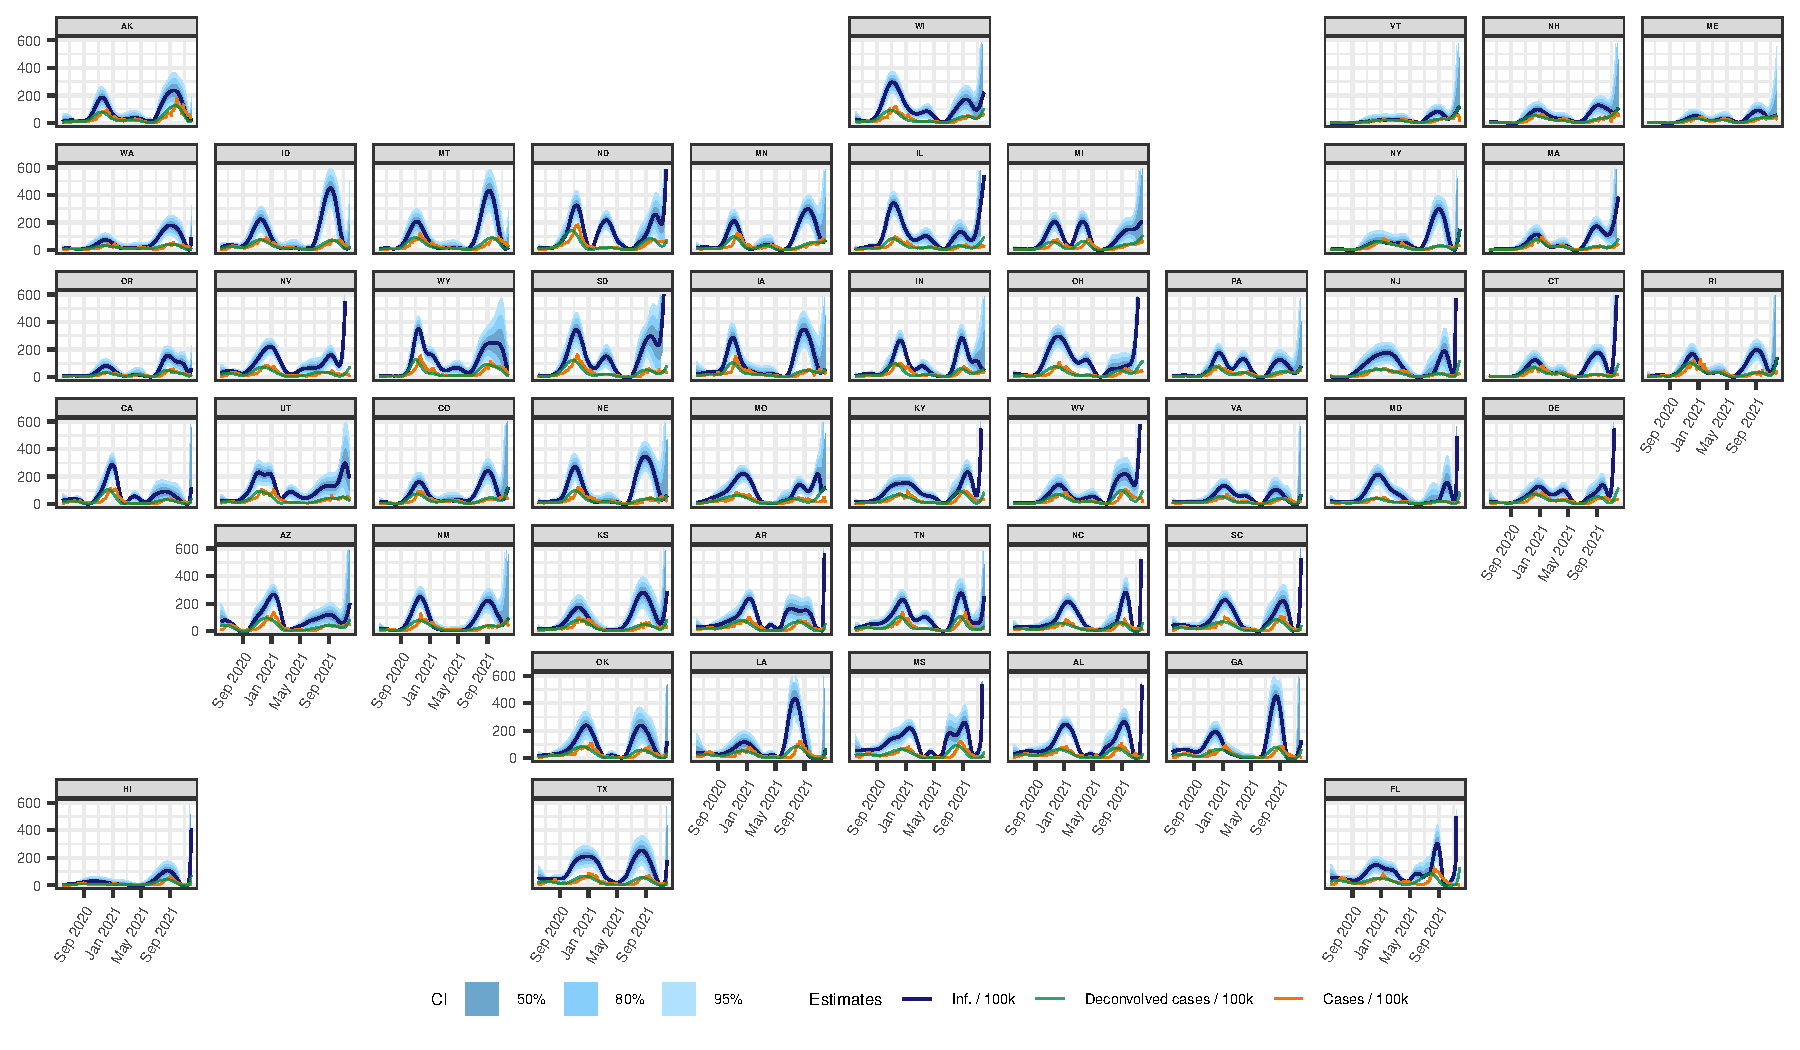
\includegraphics[width=.99\linewidth]{state_niauc_est_faceted_F24.pdf} 
\caption{Estimates of the number of daily new infections per 100,000
population for each \US state from June 1, 2020 to November 29, 2021
(dark blue line). The blue shaded regions depict the 50, 80, and 95\%
confidence intervals for the estimates, while the teal line represents
the number of new daily new deconvolved cases per 100,000, and the
dotted orange line represents the 7-day average of the new cases per
100,000.}
\label{fig:state_infect_est}
\end{figure}


\begin{figure}[!tb]
\centering
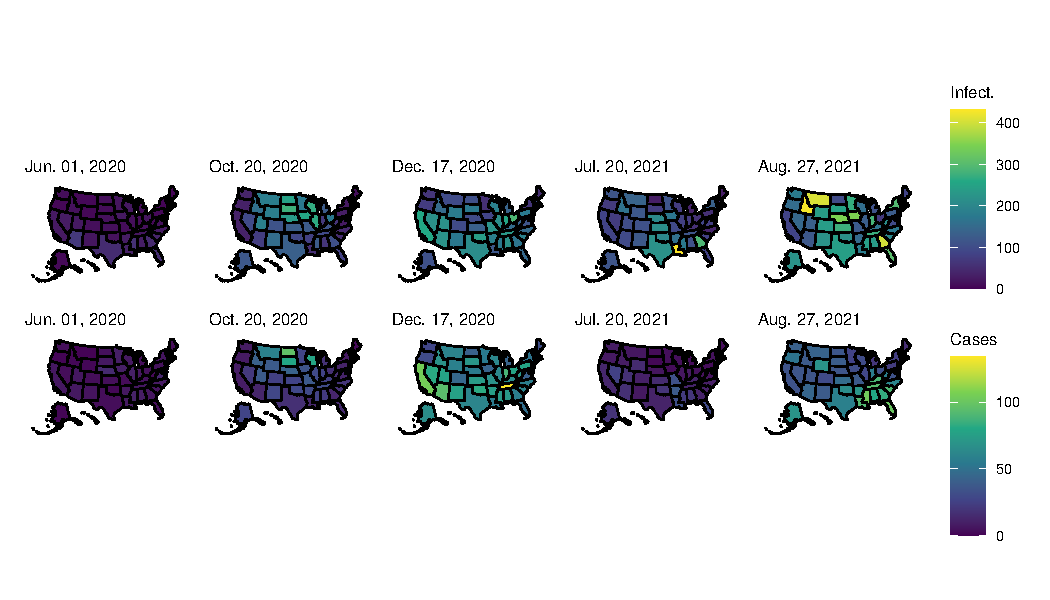
\includegraphics[width=.99\textwidth]{choro_inf_case_rates_F24.pdf}
\caption{Choropleth maps of the state-level estimates of the number of daily new
infections per $100,000$ population (top row) and the daily new cases per
$100,000$ population (bottom row) for five dates between June 1, 2020 to
November 29, 2021. Note that the first date was chosen as a baseline, while the
other dates were chosen due to having large counts of infections across all
states. In particular, the third and fifth dates present the largest number of
infections across the 50 states from each year.} 
\label{fig:choro_inf_case_rates}
\end{figure}    



    
\subsection{Infections, overall and by variant, emphasize earlier outbreaks.}
\label{sec:infections-by-voc}

\autoref{fig:six-states} examines the infection estimates for a selection of
states more closely.
The top panel shows infection estimates for these states, while the bottom panel
divides their estimated deconvolved cases based on the circulating variant
proportions at the time. From these plots, it is evident that there are times
when the total infections and the deconvolved cases broken down by the variant
categories emphasize earlier outbreaks than indicated by cases alone. For example
the major Ancestral wave for California, Maryland, Idaho, Montana, or Ohio,
peaks earlier for infections than cases. Such trends are similar with Delta,
though more obviously in Louisiana, Idaho and
Montana than California, Maryland and Ohio. The division by variant categories reveal the variant or variants
that are behind these waves. The crest-trough patterns of these by-variant
depictions align with infections rather than the cases by construction (as they
are for deconvolved cases which are re-scaled to get the infection estimates). 
\attn{These last two sentences are not sufficiently direct: they need to say something interesting, without too much mealy-mouthedness.}


\begin{figure}[!tb]
\centering
    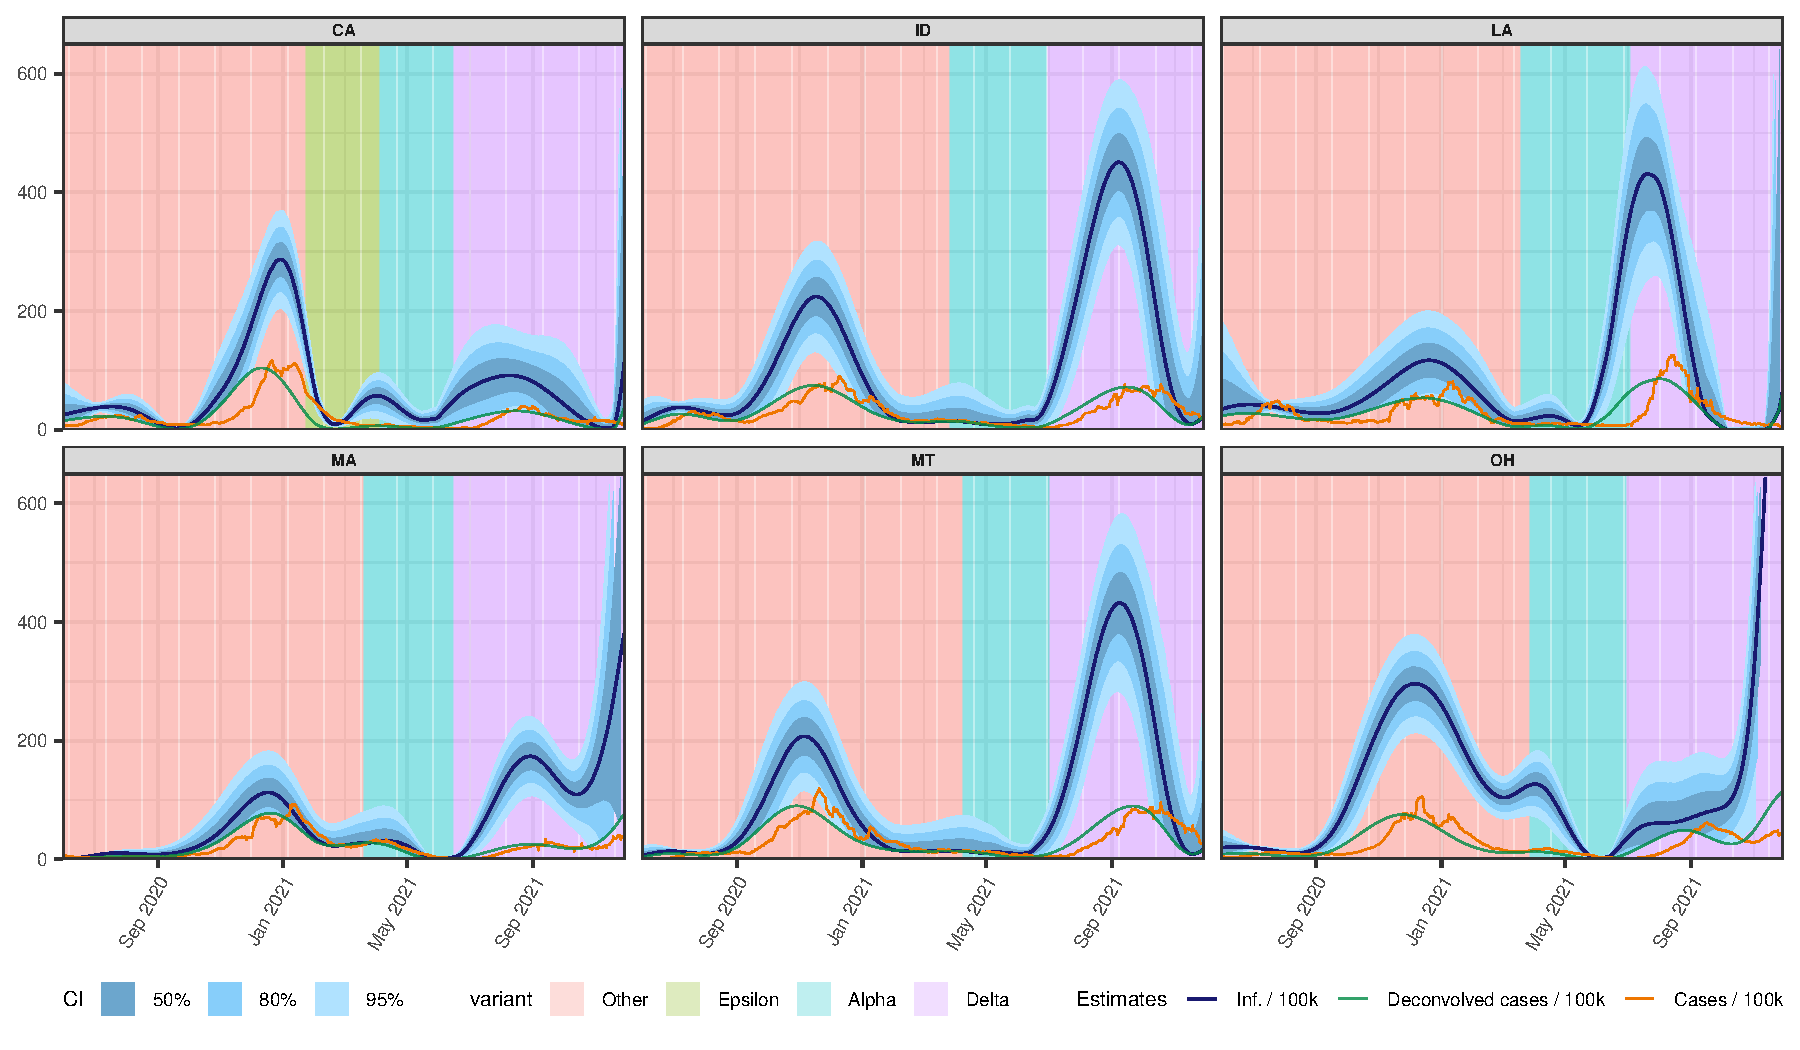
\includegraphics[width=\linewidth]{state_niauc_est_6states_F24.pdf}\\
    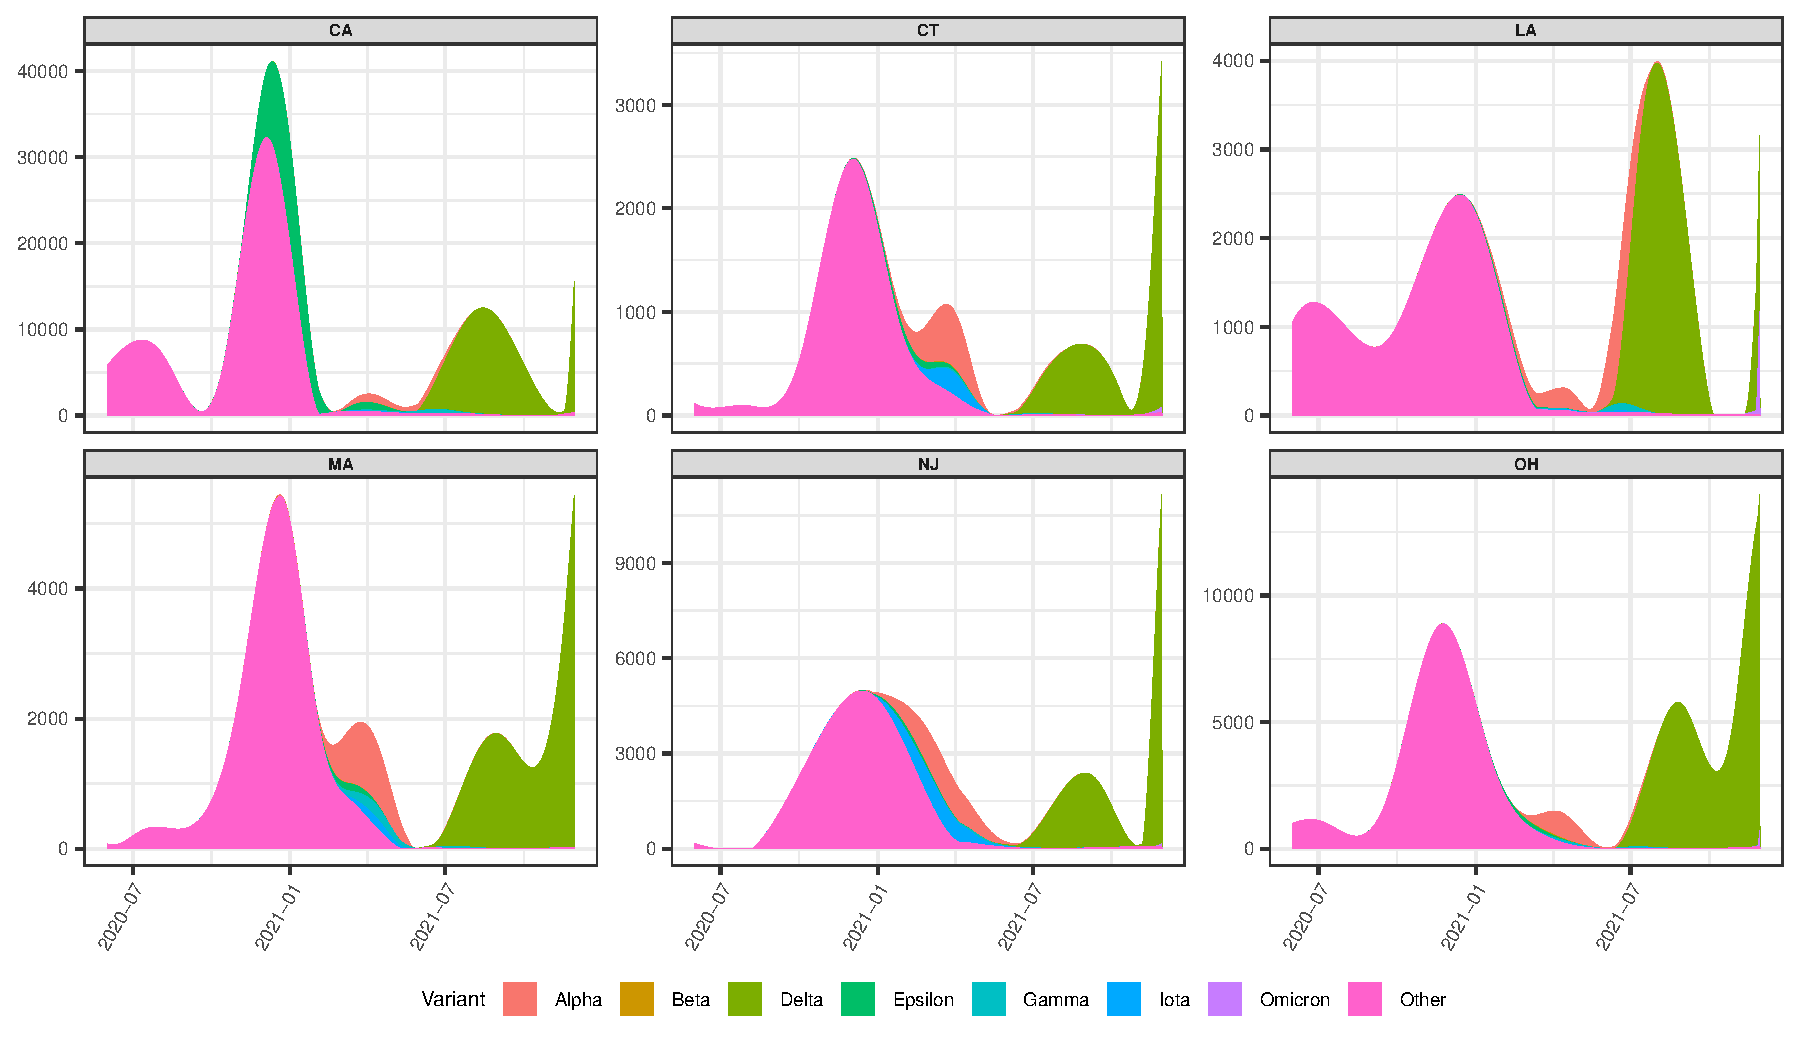
\includegraphics[width=\linewidth]{state_decon_byvar_est_6states_F24.pdf}
    \caption{Top panel: Reported cases, deconvolved cases, and estimates of
    daily new infections (dark blue line) per 100K inhabitants. The blue shaded
    regions indicate the 50, 80, and 95\% confidence bands, while the background
    is shaded to indicate the dominant variant in circulation at the time.  
    Bottom panel: Deconvolved cases colored by variant per 100K inhabitants.}
    \label{fig:six-states}
\end{figure}


\subsection{The relationship between infections and hospitalizations is complicated.}
\label{sec:lagged-correlations}

We systematically investigate the temporal relationship between infections and
hospitalizations with Spearman's rank-correlation across different lags,
shifting hospitalizations backward to align with infections
(\autoref{fig:correlations}). The maximum average correlation across states is
0.513, occurring at a lag of 13 days. In contrast, we find that the greatest
average Spearman correlation for cases is 0.691 and occurs at a lag of 1 day.
That is, case reports are nearly contemporaneous to hospitalizations, while
infection estimates clearly precede them. 

The maximum correlation at a lag of 13 days is in similar to early estimates of
the average time from infection to hospitalization of 9.7 days (95\% CI: $[5.4,
17.0]$) for cases reported in January, 2020 in Wuhan, China as well as with
estimates from across the pandemic in the UK that ranged from an average of 8.0
to 9.7 days \citep{ward2021understanding}. 

\begin{figure}[!tb]
\centering
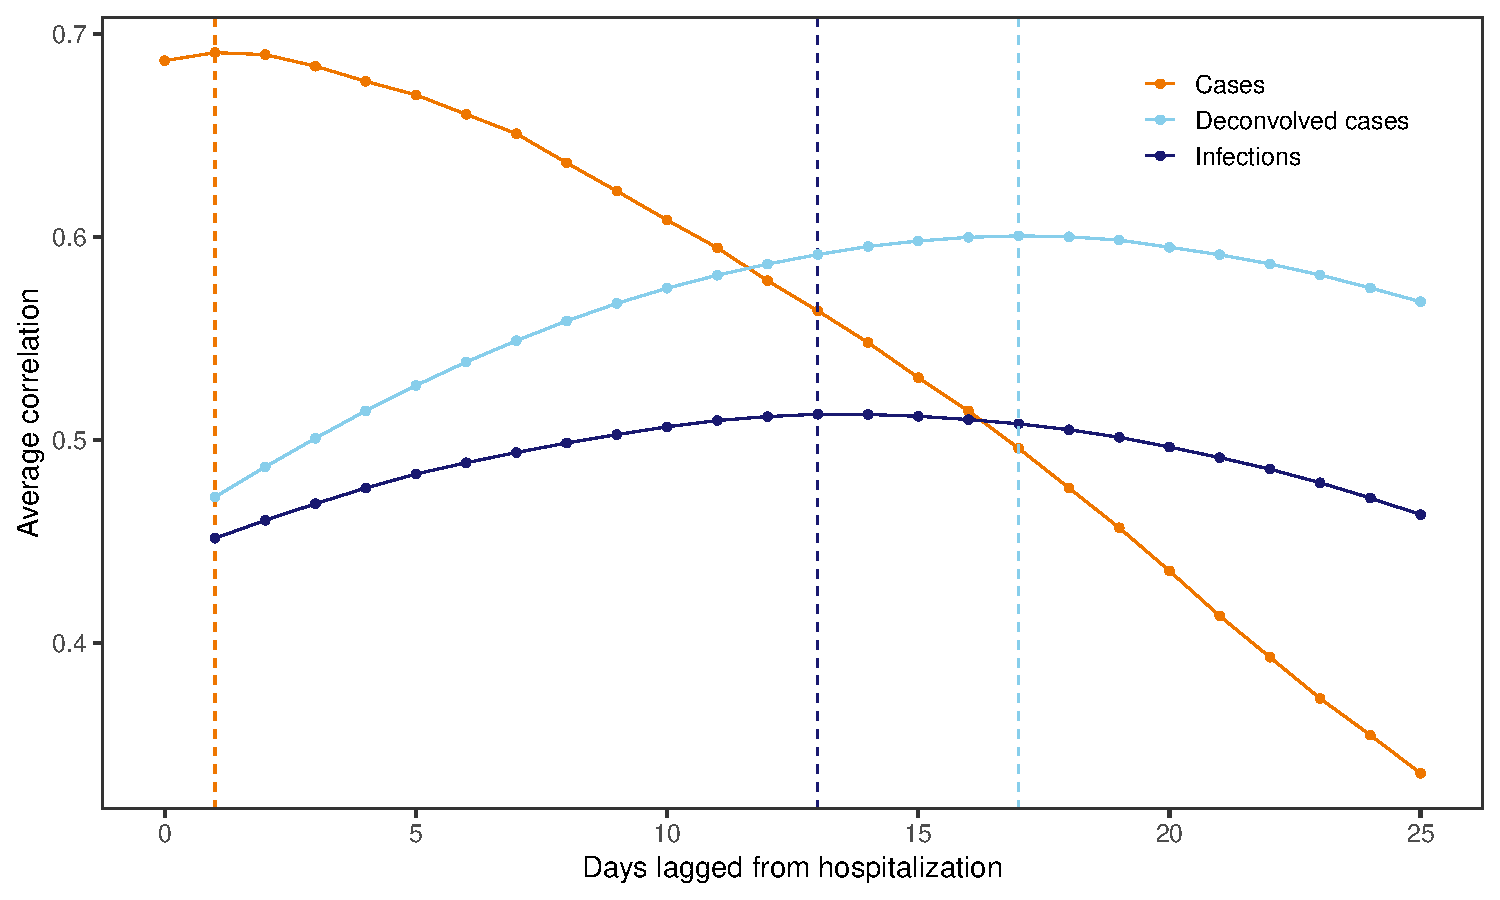
\includegraphics[width=.9\textwidth]{adj_unadj_cases_hosp_lag_corr_F24.pdf} 
\caption{Spearman's correlation between each of cases, deconvolved cases, and
infections with hospitalizations per 100,000. These are calculated for each lag,
state and rolling window of 61 days before averaging. The vertical dashed lines
indicate the lags for which the highest average correlation is attained.
\attn{Fig still wrong}}
\label{fig:correlations}
\end{figure}
    

While both the infections and deconvolved cases are leading indicators of
hospitalizations and their trajectories are similar, the average correlation
they attain is different. In particular, the correlation tends to be much
greater for deconvolved cases than for infections (with a difference of about
0.18 at the peaks). This may be due to a difference in disease severity between
the reported and unreported infections: unreported infections tend to be less
severe and less likely to lead to hospitalization than those that are reported
\citep{sallahi2021using}. Furthermore, many cases are detected contemporaneously
with hospitalization: people first test positive once they go to the emergency
room for treatment.



\subsection{Estimating infection-hospitalization ratios}
\label{sec:ihrs}

\attn{Section heading needs to state the claim (what is it?)}
As a counterpart to the correlation analysis, we compute the time-varying
infection-hospitalization ratios (IHRs) for each state using the correlation
maximizing lag. We similarly compute the case-hospitalization ratios (CHRs)
using their correlation maximizing lag for for comparison
(\autoref{fig:IHR_7dav}). 

For each state, the CHRs tend to be larger and noiser relative to
IHRs. This supports our claim that the reported infections are more
likely to require hospitalization than the unreported infections. Both the IHRs
and CHRs exhibit similar geospatial and temporal trends as are noted for
infections. Namely, states that are close in proximity (such as Ohio,
Pennsylvania, and Virginia) tend to exhibit similar patterns in the IHRs and
CHRs over time. In addition, there are similar spikes observed across many
states during waves of infections that are driven by prominent new variants. For
example, many states exhibit a striking spike in hospitalizations in mid-2021,
which coincides with the rapid takeover of the Delta variant during that time
\citep{hodcroft2021covariants}. This finding aligns with previous studies that
found an increased risk in hospitalizations with Delta in comparison to other
variants \citep{twohig2022hospital, nyberg2022comparative}. Similarly, during
the fall of 2020 there tends to be another spike in the IHRs that rivals or
surpasses that observed during the time of Delta (which is the case for states
like New York or Wyoming). 

Overall, the relationship between infections and hospitalizations is
complicated. We observe intermittent spikes that punctuate longer periods where
the IHRs tend to stabilize somewhat, in that they tend to stay below 0.1
hospitalizations per infection. Unsurprisingly, these spikes tend to align with
the emergence of new variants. 

% There does not tend to be a strict upward or downward trajectory or even a mild
% waning pattern in the IHRs, as one might expect with later variants that are
% more infectious but result in fewer hospitalization \citep{lorenzo2022covid,
% blauer2022compare}. \attn{Is the IHR actually H/I? or are the units not quite
% right (e.g., H/1M / I/100K)?}

While we computed and compared CHRs and IHRs for all states, it is important to
note that both likely vary within states and depend on confounding variables
such as age and the presence of major comorbidities
\citep{russell2023comorbidities}. Therefore, it would be beneficial to account
for such variables in their calculations by, for example, stratifying infections
and hospitalizations by age to produce age-specific estimates of the IHRs for
each state~\citep{fox2023disproportionate}.



\begin{figure}[!tb]
\centering
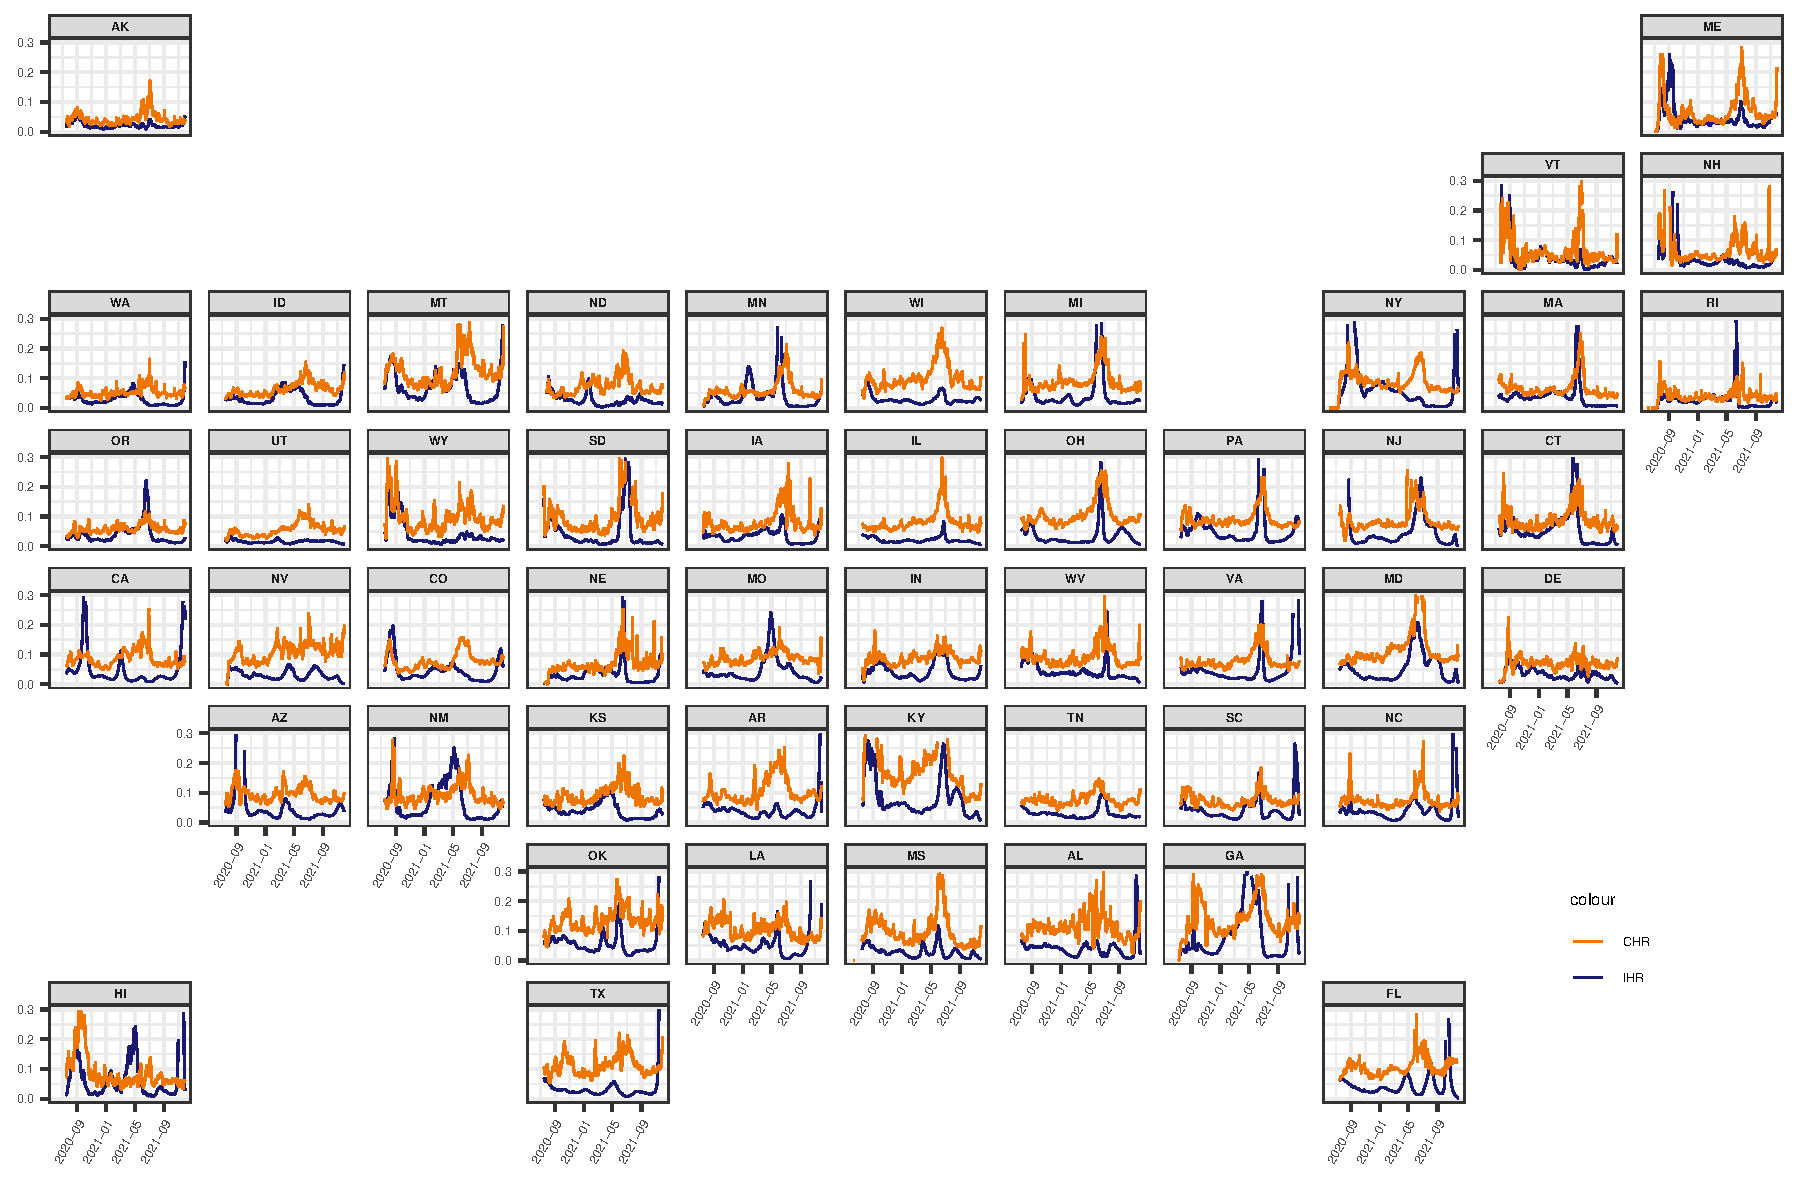
\includegraphics[width=.99\linewidth]{IHR_7dav_F24.pdf}
\caption{Time-varying IHR and CHR estimates for each state from June 1, 2020
to November 29, 2021, obtained using the corresponding optimal lag from the
systematic lag analysis. Note that the infection, case, and hospitalization
counts are subject to a center-aligned 7-day average to remove spurious day
of the week effects. Also note that the different starting points across
states are due to the availability of the hospitalization data.}
\label{fig:IHR_7dav}
\end{figure}


\subsection{Disease burden and viral transmission}

\attn{I'm not yet sure what to do with this. Some of it should go into one of 
the sections above.}

From reconstructing the time series of COVID-19 infections per $100,000$
population for each \US state from June 1, 2020 to November 29, 2021, we
observe rates of infections that vary in intensity and disease burden across
space and time (\autoref{fig:state_infect_est}, \autoref{fig:six-states}).  

Most states present at least two major spikes in infections---the first starts
in the fall of 2020 and extends into the winter season, while the second starts
in the late summer of 2021 and proceeds into the mid-fall. These represent major
waves driven by the Ancestral and Delta variants. Similar patterns in the major
surges of infections are observed in nearly all states, though to varying
degrees. In general, greater similarities in the strength and magnitude of
outbreaks are found to emerge in the clusters of states that border each other.

To avoid encroaching upon possible boundary issues with ending the estimation
during a time of volatility (the period of the Delta-Omicron transition), we
focus on the infection estimates prior to November 1, 2021. The largest observed
outbreaks prior to this time were observed in the late summer or early fall of
2021 in Georgia, Louisiana, Idaho, Montana, and Wyoming which suggests a similar
spread of the virus in small clusters of states that are in close geographic
proximity. During this time, the two states that have the highest rate of
infections per 100,000 on single day are Georgia with about $451$ infections per
100,000 on August 15, 2021 (95\% confidence interval: $[334, 567]$) and Idaho
with $451$ on September 7, 2021 (95\% confidence interval: $[312, 590]$).  Prior
to the Delta wave, the state that has the highest rate of infections per 100,000
on single day is Louisiana with about 358 infections per 100,000 on July 3, 2021
(95\% confidence interval: $[177, 539]$), followed by Wyoming with 349 on
November 13, 2020 (95\% confidence interval: $[407, 546]$).

The period of lowest viral transmission is observed in the summer and fall of
2020. During this time, the state of New Hampshire achieves the lowest weekly
rate of infections of 0.01 infections per 100,000 for the week of September 13,
2020. In the summer of 2020, Vermont maintains a rate under 10 infections per
100,000 from the week of June 1, 2020 to August 30, 2020, which is the longest
continuous stretch observed for any state.

From a brief inspection of the geo-contiguous states, we can observe similar
patterns in surges and periods of waning over time, suggesting that states who
share similarities in climate and topography performed similarly to each other.
More precisely, we can observe neighboring states such as New Hampshire and
Massachusetts or Idaho and Montana that present waves that mirror each other in
amplitude and timing. 

Interestingly, the two states that are geographically removed from the
contiguous United States, Alaska and Hawaii, tend to perform quite differently
from each other later in the pandemic. Alaska generally presents significantly
greater rates of infections than Hawaii especially during the Delta era. This
suggests that it is not so much the non-contiguity aspect as it is other
distinguishing factors that lead to lower infection rates.
